\documentclass[fontsize=13pt,oneside,headings=small,chapterprefix]{scrbook}
\usepackage{listings}
\usepackage{graphicx}
\PassOptionsToPackage{hyphens}{url}\usepackage[hidelinks]{hyperref}
\usepackage{natbib}
\usepackage{scrhack}
\usepackage{charter}
\usepackage{bookmark}
\usepackage{ucharclasses}
\usepackage{fontspec}
\usepackage{xcolor}
\usepackage{pdfpages}
\usepackage{arabxetex}
\usepackage{makeidx}

% epigraph is used to style chapter quotes
\usepackage{epigraph}
\setlength{\epigraphwidth}{.8\textwidth}
\setlength{\epigraphrule}{0pt}

\lstset{basicstyle=\ttfamily,xleftmargin=0.8em,breaklines=true,lineskip=-0.2em,aboveskip=0.8em,belowskip=0.8em}
\renewcommand*{\chapterheadstartvskip}{\vspace*{3cm}}
\date{}

\lstset{escapeinside={$<}{>$}}

\makeatletter
\lst@InputCatcodes
\def\lst@DefEC{%
 \lst@CCECUse \lst@ProcessLetter
  ^^80^^81^^82^^83^^84^^85^^86^^87^^88^^89^^8a^^8b^^8c^^8d^^8e^^8f%
  ^^90^^91^^92^^93^^94^^95^^96^^97^^98^^99^^9a^^9b^^9c^^9d^^9e^^9f%
  ^^a0^^a1^^a2^^a3^^a4^^a5^^a6^^a7^^a8^^a9^^aa^^ab^^ac^^ad^^ae^^af%
  ^^b0^^b1^^b2^^b3^^b4^^b5^^b6^^b7^^b8^^b9^^ba^^bb^^bc^^bd^^be^^bf%
  ^^c0^^c1^^c2^^c3^^c4^^c5^^c6^^c7^^c8^^c9^^ca^^cb^^cc^^cd^^ce^^cf%
  ^^d0^^d1^^d2^^d3^^d4^^d5^^d6^^d7^^d8^^d9^^da^^db^^dc^^dd^^de^^df%
  ^^e0^^e1^^e2^^e3^^e4^^e5^^e6^^e7^^e8^^e9^^ea^^eb^^ec^^ed^^ee^^ef%
  ^^f0^^f1^^f2^^f3^^f4^^f5^^f6^^f7^^f8^^f9^^fa^^fb^^fc^^fd^^fe^^ff%
  тявΧαίρετΑΊΡΤΕ“”
  ^^00}
\lst@RestoreCatcodes
\makeatother

\setcounter{secnumdepth}{0}
\setcounter{tocdepth}{1}
\setmonofont[Scale=0.8]{Inconsolata LGC}
\defaultfontfeatures[\emojifont]{Scale=1.15}
\newfontface{\emojifont}{Symbola_hint.ttf}
\newfontfamily{\cjkfont}{TW-Sung}
\setTransitionsFor{MiscellaneousSymbolsAndPictographs}{\emojifont}{\normalfont}{}

\newfontfamily{\cinzel}{Cinzel}
\setkomafont{disposition}{\bfseries\cinzel}
\definecolor{silver-chalice}{HTML}{AAAAAA}
\setkomafont{chapterprefix}{\small\color{silver-chalice}}
\RedeclareSectionCommand[innerskip=0pt]{chapter}

\pagestyle{plain}

\usepackage{newunicodechar}
\newunicodechar{π}{$\pi$}
\newunicodechar{ϕ}{$\varphi$}
\newunicodechar{≈}{$\approx$}
\newunicodechar{β}{\ss}
\newunicodechar{⮪}{\emojifont{⮪}}

\graphicspath{{../}}
\definecolor{coveryellow}{rgb}{0.997,0.840,0.122}

\makeindex

\begin{document}

\pagecolor{coveryellow}
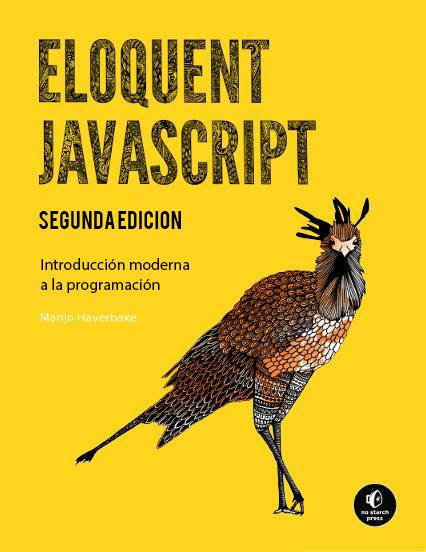
\includepdf{../img/cover.jpg}
\pagecolor{white}

\author{Marijn Haverbeke}

\title{Eloquent JavaScript}

\subtitle{3rd edition}

\maketitle

\frontmatter

  \noindent Copyright \textcopyright{} 2018 by Marijn Haverbeke

  \vskip 1em

  \noindent This work is licensed under a Creative Commons
  attribution-noncommercial license
  (\url{http://creativecommons.org/licenses/by-nc/3.0/}). All code in
  the book may also be considered licensed under an MIT license
  (\url{http://opensource.org/licenses/MIT}).

  The illustrations are contributed by various artists: Cover by
  Madalina Tantareanu. Octopus in Chapter 2 by Jim Tierney. Pixel art
  in Chapters 7 and 16 by Antonio Perdomo Pastor. Regular expression
  diagrams in Chapter 9 generated with
  \href{http://regexper.com}{regexper.com} by Jeff Avallone. Village
  photograph in Chapter 11 by Fabrice Creuzot. Game concept for
  Chapter 15 by \href{http://lessmilk.com}{Thomas Palef}.

  The third edition of Eloquent JavaScript was made possible
  by \href{http://eloquentjavascript.net/backers3.html}{325 financial backers}.

  \vskip 1em

  \noindent You can buy a print version of this book, with an extra
  bonus chapter included, printed by No Starch Press at
  \url{https://www.amazon.com/Eloquent-JavaScript-2nd-Ed-Introduction/dp/1593275846}.

\tableofcontents

\mainmatter

\input{00_intro.tex}

\input{01_values.tex}

\input{02_program_structure.tex}

\input{03_functions.tex}

\input{04_data.tex}

\input{05_higher_order.tex}

\input{06_object.tex}

\input{07_robot.tex}

\input{08_error.tex}

\input{09_regexp.tex}

\input{10_modules.tex}

\input{11_async.tex}

\input{12_language.tex}

\input{13_browser.tex}

\input{14_dom.tex}

\input{15_event.tex}

\input{16_game.tex}

\input{17_canvas.tex}

\input{18_http.tex}

\input{19_paint.tex}

\input{20_node.tex}

\input{21_skillsharing.tex}

\input{hints.tex}

\backmatter

\printindex

\end{document}
